%%%%%%%%%%%%%%%%%%%%%%%%%%%%%%%%%%%%%%%%%%%%%%%%%%%%%%%%%%%%%%%%%%%%%%%%%%%%%%%%%%%%%%%%
%%
%%  Última alteração em 08/2013 por Rafael Pasquini (WTDCC 2013)
%%
%%%%%%%%%%%%%%%%%%%%%%%%%%%%%%%%%%%%%%%%%%%%%%%%%%%%%%%%%%%%%%%%%%%%%%%%%%%%%%%%%%%%%%%%

\documentclass[11pt]{article}
\usepackage{sbc-template}
\usepackage{graphicx,url}
%\usepackage[dvips]{graphicx}
%\usepackage[pdftex]{color,graphicx}
\usepackage{multicol}
\usepackage{multirow}
\usepackage{verbatim}
\usepackage{array}
\usepackage{amssymb,amsmath}
\usepackage[brazilian]{babel}
\usepackage[utf8]{inputenc}
\usepackage[T1]{fontenc}
\usepackage{tabularx}
 \usepackage[table,xcdraw]{xcolor}

\sloppy

\title{3$^o$ Trabalho de Inteligência Computacional - Rede Neural}

\author{Autor: Gustavo Rezende Silva,\\ Orientador:Gina Maira Barbosa
de Oliveira}


\address{Faculdade de Computação\\
 Universidade Federal do Uberlândia (UFU)\\
  Uberlândia -- MG -- Brasil
  \email{gustavorezendesilva@hotmail.com, gina@ufu.br}
}

\begin{document}

\maketitle


\begin{resumo}
Este trabalho tem como intuito desenvolver uma rede neural do tipo Perceptron
para aprender os padrões de 6 matrizes 6x5 distintas. Estas representam os números
entre 0 e 5.
\end{resumo}

\begin{palavraschave}
rede neural, perceptron, inteligência computacional
\end{palavraschave}

\section{Introdução}
\label{sec:intro}

Este trabalho tem como intuito desenvolver uma rede neural do tipo Perceptron
para aprender os padrões de 6 matrizes 6x5 distintas (fig. \ref{fig:patterns}),
estas representam os números entre 0 e 5. Além disso, demonstrar para o aluno
através da prática como realizar o treinamento de neurônios e a plasticidade,
capacidade de identificar padrões parecidos com os utilizados no treinamento, dos
mesmos.

\begin{figure}[h]
  \centering
  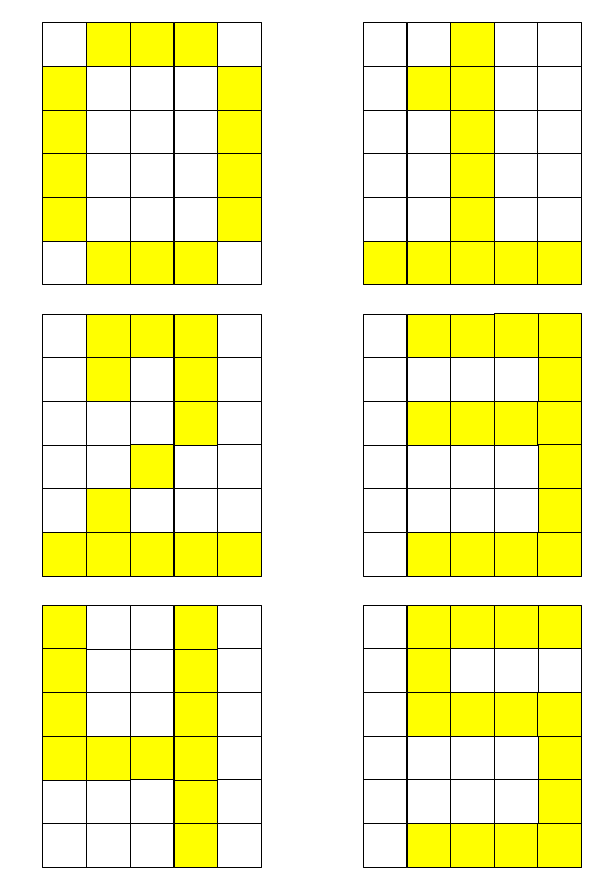
\includegraphics[width=8cm]{patterns.png}
  \caption{Padrões que devem ser aprendidos}
  \label{fig:patterns}
\end{figure}

\section{Desenvolvimento}
\label{sec:desen}
Para iniciar o desenvolvimento foi necessário definir quais seriam as entradas
de um neurônio, função de ativação, e saída.

Uma vez que cada padrão possui 30 quadrados foi definido que cada um seria uma
entrada do neurônio (fig. \ref{fig:matriz}), além disso existe uma entrada que é
sempre positiva e é chamada de bias. O neurônio é representado como na
fig. \ref{fig:neuron}

A função de ativação adotada foi a degrau unitário, ou seja, caso o valor da soma das
entradas seja menor ou igual a $0$ a saída é $0$, e se a soma das entradas for maior que $1$
o resultado é $1$. Com isso, $Y1$ pode assumir os valores $0$ ou $1$ e sua
interpretação varia de acordo com o treinamento aplicado. Por fim, o neurônio foi
representado como na fig. \ref{fig:neuron}

\begin{figure}[h]
  \centering
  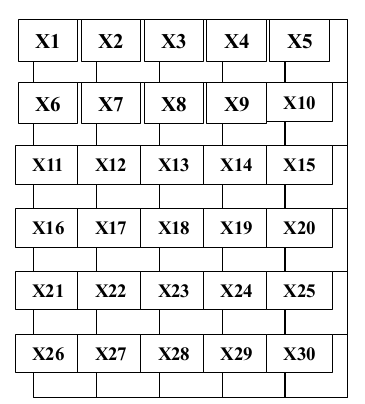
\includegraphics[width=5cm]{matriz.png}
  \caption{Representação das entradas}
  \label{fig:matriz}
\end{figure}

\begin{figure}[h]
  \centering
  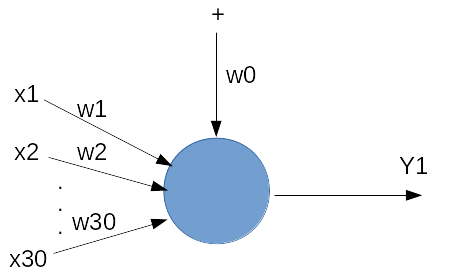
\includegraphics[width=5cm]{neuron.png}
  \caption{Representação de um neurônio}
  \label{fig:neuron}
\end{figure}

Inicialmente foi treinado apenas um neurônio com o intuito de
aprender os padrões dos números 0 e 1 (fig. \ref{fig:patterns}), de forma que
$Y1$ é $0$ caso o padrão represente um $0$ e $1$ se representar $1$.

O treinamento foi realizado para os pesos inciais iguais a zero e com pesos iniciais
aleatórios. Para ambos os casos foram necessáras 3 épocas para encontrar acabar
de treinar, os resultados se encontram nas tabelas \ref{tab:1w0} e \ref{tab:1wr}.

\begin{table}[h]
  \centering
  \caption{Pesos da etapa 1 a partir de pesos iniciais zerados}
  \label{tab:1w0}
  \begin{tabular}{lllll}
  \cellcolor[HTML]{000000}{\color[HTML]{FFFFFF} W0} &                            &                            &                            &                            \\
  0                                                 &                            &                            &                            &                            \\
  \rowcolor[HTML]{000000}
  {\color[HTML]{FFFFFF} W1}                         & {\color[HTML]{FFFFFF} W2}  & {\color[HTML]{FFFFFF} W3}  & {\color[HTML]{FFFFFF} W4}  & {\color[HTML]{FFFFFF} W5}  \\
  0                                                 & -1                         & 0                          & -1                         & 0                          \\
  \rowcolor[HTML]{000000}
  {\color[HTML]{FFFFFF} W6}                         & {\color[HTML]{FFFFFF} W7}  & {\color[HTML]{FFFFFF} W8}  & {\color[HTML]{FFFFFF} W9}  & {\color[HTML]{FFFFFF} W10} \\
  -1                                                & 1                          & 1                          & 0                          & -1                         \\
  \rowcolor[HTML]{000000}
  {\color[HTML]{FFFFFF} W11}                        & {\color[HTML]{FFFFFF} W12} & {\color[HTML]{FFFFFF} W13} & {\color[HTML]{FFFFFF} W14} & {\color[HTML]{FFFFFF} W15} \\
  -1                                                & 0                          & 1                          & 0                          & -1                         \\
  \rowcolor[HTML]{000000}
  {\color[HTML]{FFFFFF} W16}                        & {\color[HTML]{FFFFFF} W17} & {\color[HTML]{FFFFFF} W18} & {\color[HTML]{FFFFFF} W19} & {\color[HTML]{FFFFFF} W20} \\
  -1                                                & 0                          & 1                          & 0                          & -1                         \\
  \rowcolor[HTML]{000000}
  {\color[HTML]{FFFFFF} W21}                        & {\color[HTML]{FFFFFF} W22} & {\color[HTML]{FFFFFF} W23} & {\color[HTML]{FFFFFF} W24} & {\color[HTML]{FFFFFF} W25} \\
  -1                                                & 0                          & 1                          & 0                          & -1                         \\
  \rowcolor[HTML]{000000}
  {\color[HTML]{FFFFFF} W26}                        & {\color[HTML]{FFFFFF} W27} & {\color[HTML]{FFFFFF} W28} & {\color[HTML]{FFFFFF} W29} & {\color[HTML]{FFFFFF} W30} \\
  1                                                 & 0                          & 0                          & 0                          & 1
  \end{tabular}
\end{table}

\begin{table}[h]
  \centering
  \caption{Pesos da etapa 1 a partir de pesos iniciais aleatórios}
  \label{tab:1wr}
  \begin{tabular}[width=8cm]{lllll}
  \cellcolor[HTML]{000000}{\color[HTML]{FFFFFF} w0} &                            &                            &                            &                            \\
  0.605                                             &                            &                            &                            &                            \\
  \rowcolor[HTML]{000000}
  {\color[HTML]{FFFFFF} w1}                         & {\color[HTML]{FFFFFF} w2}  & {\color[HTML]{FFFFFF} w3}  & {\color[HTML]{FFFFFF} w4}  & {\color[HTML]{FFFFFF} w5}  \\
  1.083                                             & -1.957                     & -0.836                     & 1.744                      & -1.29                      \\
  \rowcolor[HTML]{000000}
  {\color[HTML]{FFFFFF} w6}                         & {\color[HTML]{FFFFFF} w7}  & {\color[HTML]{FFFFFF} w8}  & {\color[HTML]{FFFFFF} w9}  & {\color[HTML]{FFFFFF} w10} \\
  -2.563                                            & -0.345                     & -0.894                     & -2.162                     & 0.058                      \\
  \rowcolor[HTML]{000000}
  {\color[HTML]{FFFFFF} w11}                        & {\color[HTML]{FFFFFF} w12} & {\color[HTML]{FFFFFF} w13} & {\color[HTML]{FFFFFF} w14} & {\color[HTML]{FFFFFF} w15} \\
  0.068                                             & 1.047                      & 3.455                      & 1.113                      & 1.812                      \\
  \rowcolor[HTML]{000000}
  {\color[HTML]{FFFFFF} w16}                        & {\color[HTML]{FFFFFF} w17} & {\color[HTML]{FFFFFF} w18} & {\color[HTML]{FFFFFF} w19} & {\color[HTML]{FFFFFF} w20} \\
  -2.484                                            & 1.291                      & 2.234                      & 2.871                      & -0.661                     \\
  \rowcolor[HTML]{000000}
  {\color[HTML]{FFFFFF} w21}                        & {\color[HTML]{FFFFFF} w22} & {\color[HTML]{FFFFFF} w23} & {\color[HTML]{FFFFFF} w24} & {\color[HTML]{FFFFFF} w25} \\
  -0.661                                            & 0.601                      & 1.582                      & 2.319                      & -0.881                     \\
  \rowcolor[HTML]{000000}
  {\color[HTML]{FFFFFF} w26}                        & {\color[HTML]{FFFFFF} w27} & {\color[HTML]{FFFFFF} w28} & {\color[HTML]{FFFFFF} w29} & {\color[HTML]{FFFFFF} w30} \\
  1.969                                             & -1.088                     & -0.072                     & -0.644                     & 3.647
  \end{tabular}
\end{table}

Após realizar o treinamento o neurônio foi testado com algumas variações do
padrão 0 e 1, e foi concluído que para variações não grosseiras o resultado é
satisfatório. E ainda, testou-se com todos os padrões dos númeoros de 0 até 5 e
os resultados se encontram na tabela \ref{tab:res01_1}.

\begin{table}[h]
  \centering
  \caption{Resultados da etapa 1 para os padrões entre 0 e 5}
  \label{tab:res01_1}
  \begin{tabular}{llllllll}
  \rowcolor[HTML]{000000}
  {\color[HTML]{FFFFFF} Padrão}                            & {\color[HTML]{FFFFFF} 0} & {\color[HTML]{FFFFFF} 1} & {\color[HTML]{FFFFFF} 2} & {\color[HTML]{FFFFFF} 3} & {\color[HTML]{FFFFFF} 4} & {\color[HTML]{FFFFFF} 5} & {\color[HTML]{FFFFFF} 6} \\
  \cellcolor[HTML]{000000}{\color[HTML]{FFFFFF} Resultado} & 0                        & 1                        & 1                        & 1                        & 1                        & 1                        & 1
  \end{tabular}
\end{table}

Na etapa seguinte foi treinado dois neurônios, o primeiro para aprender o número zero e
outro para aprender o número um. A saída deve ser $0$ caso o padrão de entrada
não represente o número a ser aprendido por aquele neurônio e $1$ se representar.

Novamente o treinamento foi executado para pesos iniciais zerados e aleatórios e
suas épocas anotadas. Os resultados se encontram entre as tabelas \ref{tab:epoca_2}
e \ref{tab:wp1r_2}.

\begin{table}[h]
  \centering
  \caption{Numero de épocas necessárias}
  \label{tab:epoca_2}
  \begin{tabular}{lll}
  \rowcolor[HTML]{000000}
  {\color[HTML]{FFFFFF} Pesos Iniciais} & {\color[HTML]{FFFFFF} Neurônio} & {\color[HTML]{FFFFFF} Épocas} \\
  Zerados                               & 0                               & 2                             \\
  Zerados                               & 1                               & 3                             \\
  Aleatórios                            & 0                               & 2                             \\
  Aleatórios                            & 1                               & 2
  \end{tabular}
\end{table}

\begin{table}[h]
  \centering
  \caption{Pesos da etapa 2 a partir de pesos iniciais zerado para o número zero}
  \label{tab:wp0z_2}
  \begin{tabular}{lllll}
  \cellcolor[HTML]{000000}{\color[HTML]{FFFFFF} W0} &                            &                            &                            &                            \\
  0                                                 &                            &                            &                            &                            \\
  \rowcolor[HTML]{000000}
  {\color[HTML]{FFFFFF} W1}                         & {\color[HTML]{FFFFFF} W2}  & {\color[HTML]{FFFFFF} W3}  & {\color[HTML]{FFFFFF} W4}  & {\color[HTML]{FFFFFF} W5}  \\
  0                                                 & 1                          & 0                          & 1                          & 0                          \\
  \rowcolor[HTML]{000000}
  {\color[HTML]{FFFFFF} W6}                         & {\color[HTML]{FFFFFF} W7}  & {\color[HTML]{FFFFFF} W8}  & {\color[HTML]{FFFFFF} W9}  & {\color[HTML]{FFFFFF} W10} \\
  1                                                 & -1                         & -1                         & 0                          & 1                          \\
  \rowcolor[HTML]{000000}
  {\color[HTML]{FFFFFF} W11}                        & {\color[HTML]{FFFFFF} W12} & {\color[HTML]{FFFFFF} W13} & {\color[HTML]{FFFFFF} W14} & {\color[HTML]{FFFFFF} W15} \\
  1                                                 & 0                          & -1                         & 0                          & 1                          \\
  \rowcolor[HTML]{000000}
  {\color[HTML]{FFFFFF} W16}                        & {\color[HTML]{FFFFFF} W17} & {\color[HTML]{FFFFFF} W18} & {\color[HTML]{FFFFFF} W19} & {\color[HTML]{FFFFFF} W20} \\
  1                                                 & 0                          & -1                         & 0                          & 1                          \\
  \rowcolor[HTML]{000000}
  {\color[HTML]{FFFFFF} W21}                        & {\color[HTML]{FFFFFF} W22} & {\color[HTML]{FFFFFF} W23} & {\color[HTML]{FFFFFF} W24} & {\color[HTML]{FFFFFF} W25} \\
  1                                                 & 0                          & -1                         & 0                          & 1                          \\
  \rowcolor[HTML]{000000}
  {\color[HTML]{FFFFFF} W26}                        & {\color[HTML]{FFFFFF} W27} & {\color[HTML]{FFFFFF} W28} & {\color[HTML]{FFFFFF} W29} & {\color[HTML]{FFFFFF} W30} \\
  -1                                                & 0                          & 0                          & 0                          & -1
  \end{tabular}
\end{table}

\begin{table}[h]
  \centering
  \caption{Pesos da etapa 2 a partir de pesos iniciais zerado para o número um}
  \label{tab:wp1z_2}
  \begin{tabular}{lllll}
  \cellcolor[HTML]{000000}{\color[HTML]{FFFFFF} W0} &                            &                            &                            &                            \\
  0                                                 &                            &                            &                            &                            \\
  \rowcolor[HTML]{000000}
  {\color[HTML]{FFFFFF} W1}                         & {\color[HTML]{FFFFFF} W2}  & {\color[HTML]{FFFFFF} W3}  & {\color[HTML]{FFFFFF} W4}  & {\color[HTML]{FFFFFF} W5}  \\
  0                                                 & -1                         & 0                          & -1                         & 0                          \\
  \rowcolor[HTML]{000000}
  {\color[HTML]{FFFFFF} W6}                         & {\color[HTML]{FFFFFF} W7}  & {\color[HTML]{FFFFFF} W8}  & {\color[HTML]{FFFFFF} W9}  & {\color[HTML]{FFFFFF} W10} \\
  -1                                                & 1                          & 1                          & 0                          & -1                         \\
  \rowcolor[HTML]{000000}
  {\color[HTML]{FFFFFF} W11}                        & {\color[HTML]{FFFFFF} W12} & {\color[HTML]{FFFFFF} W13} & {\color[HTML]{FFFFFF} W14} & {\color[HTML]{FFFFFF} W15} \\
  -1                                                & 0                          & 1                          & 0                          & -1                         \\
  \rowcolor[HTML]{000000}
  {\color[HTML]{FFFFFF} W16}                        & {\color[HTML]{FFFFFF} W17} & {\color[HTML]{FFFFFF} W18} & {\color[HTML]{FFFFFF} W19} & {\color[HTML]{FFFFFF} W20} \\
  -1                                                & 0                          & 1                          & 0                          & -1                         \\
  \rowcolor[HTML]{000000}
  {\color[HTML]{FFFFFF} W21}                        & {\color[HTML]{FFFFFF} W22} & {\color[HTML]{FFFFFF} W23} & {\color[HTML]{FFFFFF} W24} & {\color[HTML]{FFFFFF} W25} \\
  -1                                                & 0                          & 1                          & 0                          & -1                         \\
  \rowcolor[HTML]{000000}
  {\color[HTML]{FFFFFF} W26}                        & {\color[HTML]{FFFFFF} W27} & {\color[HTML]{FFFFFF} W28} & {\color[HTML]{FFFFFF} W29} & {\color[HTML]{FFFFFF} W30} \\
  1                                                 & 0                          & 0                          & 0                          & 1
  \end{tabular}
\end{table}

\begin{table}[h]
  \centering
  \caption{Pesos da etapa 2 a partir de pesos iniciais aleatórios para o número zero}
  \label{tab:wp0r_2}
  \begin{tabular}{lllll}
  \cellcolor[HTML]{000000}{\color[HTML]{FFFFFF} W0} &                            &                            &                            &                            \\
  -0.261                                            &                            &                            &                            &                            \\
  \rowcolor[HTML]{000000}
  {\color[HTML]{FFFFFF} W1}                         & {\color[HTML]{FFFFFF} W2}  & {\color[HTML]{FFFFFF} W3}  & {\color[HTML]{FFFFFF} W4}  & {\color[HTML]{FFFFFF} W5}  \\
  2.439                                             & -1.311                     & 0.903                      & 1.389                      & -0.601                     \\
  \rowcolor[HTML]{000000}
  {\color[HTML]{FFFFFF} W6}                         & {\color[HTML]{FFFFFF} W7}  & {\color[HTML]{FFFFFF} W8}  & {\color[HTML]{FFFFFF} W9}  & {\color[HTML]{FFFFFF} W10} \\
  1.546                                             & -1.75                      & -3.289                     & 1.384                      & -1.693                     \\
  \rowcolor[HTML]{000000}
  {\color[HTML]{FFFFFF} W11}                        & {\color[HTML]{FFFFFF} W12} & {\color[HTML]{FFFFFF} W13} & {\color[HTML]{FFFFFF} W14} & {\color[HTML]{FFFFFF} W15} \\
  0.985                                             & -0.57                      & 0.762                      & -1.903                     & -1.553                     \\
  \rowcolor[HTML]{000000}
  {\color[HTML]{FFFFFF} W16}                        & {\color[HTML]{FFFFFF} W17} & {\color[HTML]{FFFFFF} W18} & {\color[HTML]{FFFFFF} W19} & {\color[HTML]{FFFFFF} W20} \\
  2.485                                             & 0.595                      & -0.318                     & 1.355                      & -1.067                     \\
  \rowcolor[HTML]{000000}
  {\color[HTML]{FFFFFF} W21}                        & {\color[HTML]{FFFFFF} W22} & {\color[HTML]{FFFFFF} W23} & {\color[HTML]{FFFFFF} W24} & {\color[HTML]{FFFFFF} W25} \\
  3.925                                             & -1.044                     & -2.279                     & 0.449                      & 1.281                      \\
  \rowcolor[HTML]{000000}
  {\color[HTML]{FFFFFF} W26}                        & {\color[HTML]{FFFFFF} W27} & {\color[HTML]{FFFFFF} W28} & {\color[HTML]{FFFFFF} W29} & {\color[HTML]{FFFFFF} W30} \\
  0.69                                              & 1.361                      & 0.415                      & 1.253                      & -0.993
  \end{tabular}
\end{table}

\begin{table}[h]
  \centering
  \caption{Pesos da etapa 2 a partir de pesos iniciais aleatórios para o número um}
  \label{tab:wp1r_2}
  \begin{tabular}{lllll}
  \cellcolor[HTML]{000000}{\color[HTML]{FFFFFF} W0} &                            &                            &                            &                            \\
  -1.847                                            &                            &                            &                            &                            \\
  \rowcolor[HTML]{000000}
  {\color[HTML]{FFFFFF} W1}                         & {\color[HTML]{FFFFFF} W2}  & {\color[HTML]{FFFFFF} W3}  & {\color[HTML]{FFFFFF} W4}  & {\color[HTML]{FFFFFF} W5}  \\
  0.691                                             & -1.098                     & 0.263                      & -1.921                     & -0.493                     \\
  \rowcolor[HTML]{000000}
  {\color[HTML]{FFFFFF} W6}                         & {\color[HTML]{FFFFFF} W7}  & {\color[HTML]{FFFFFF} W8}  & {\color[HTML]{FFFFFF} W9}  & {\color[HTML]{FFFFFF} W10} \\
  2.809                                             & 1.33                       & 1.218                      & -0.601                     & -1.157                     \\
  \rowcolor[HTML]{000000}
  {\color[HTML]{FFFFFF} W11}                        & {\color[HTML]{FFFFFF} W12} & {\color[HTML]{FFFFFF} W13} & {\color[HTML]{FFFFFF} W14} & {\color[HTML]{FFFFFF} W15} \\
  -2.798                                            & 0.035                      & 2.812                      & 2.507                      & 0.483                      \\
  \rowcolor[HTML]{000000}
  {\color[HTML]{FFFFFF} W16}                        & {\color[HTML]{FFFFFF} W17} & {\color[HTML]{FFFFFF} W18} & {\color[HTML]{FFFFFF} W19} & {\color[HTML]{FFFFFF} W20} \\
  0.296                                             & -1.693                     & -0.836                     & -1.35                      & -2.554                     \\
  \rowcolor[HTML]{000000}
  {\color[HTML]{FFFFFF} W21}                        & {\color[HTML]{FFFFFF} W22} & {\color[HTML]{FFFFFF} W23} & {\color[HTML]{FFFFFF} W24} & {\color[HTML]{FFFFFF} W25} \\
  2.295                                             & -1.188                     & 0.167                      & -0.256                     & 0.3                        \\
  \rowcolor[HTML]{000000}
  {\color[HTML]{FFFFFF} W26}                        & {\color[HTML]{FFFFFF} W27} & {\color[HTML]{FFFFFF} W28} & {\color[HTML]{FFFFFF} W29} & {\color[HTML]{FFFFFF} W30} \\
  3.064                                             & -0.896                     & -1.286                     & 1.316                      & 0.318
  \end{tabular}
\end{table}

Em seguida, os neurônios foram testados novamente com algumas variações do
padrão 0 e 1, notou-se que o resultado foi igual ao da primeira etapa. Então, os
padrões entre 0 e 5 foram testados e se encontram na tabela \ref{tab:res01_2}

\begin{table}[]
\centering
\caption{Resultados da etapa 2 para os padrões entre 0 e 5}
\label{tab:res01_2}
\begin{tabular}{lll}
\rowcolor[HTML]{000000}
{\color[HTML]{FFFFFF} Padrão} & {\color[HTML]{FFFFFF} Neurônio 0} & {\color[HTML]{FFFFFF} Neurônio 1} \\
0                             & 1                                 & 0                                 \\
1                             & 0                                 & 1                                 \\
2                             & 0                                 & 1                                 \\
3                             & 1                                 & 0                                 \\
4                             & 1                                 & 0                                 \\
5                             & 1                                 & 0
\end{tabular}
\end{table}

Na última fase 6 neurônios foram treinados, cada um deve aprender um número
diferente entre 0 e 5. A saída deve ser $1$ caso a entrada represente o padrão
de treinamento e $0$ se não representar.

Mais uma vez treinou-se os neurônios para pesos iniciais zerados e aleatórios e
suas épocas foram anotadas. Os resultados se encontram entre as tabelas \ref{tab:epoca_3}
e \ref{tab:wp5z_3}.

\begin{table}[h]
\centering
\caption{Numero de épocas necessárias}
\label{tab:epoca_3}
\begin{tabular}{lll}
\multicolumn{1}{c}{}                                    & \cellcolor[HTML]{000000}{\color[HTML]{FFFFFF} Zerados} & \cellcolor[HTML]{000000}{\color[HTML]{FFFFFF} Aleatórios} \\
\cellcolor[HTML]{000000}{\color[HTML]{FFFFFF} Neurônio} & Épocas                                                 & Épocas                                                    \\
\cellcolor[HTML]{000000}{\color[HTML]{FFFFFF} 0}        & 3                                                      & 3                                                         \\
\cellcolor[HTML]{000000}{\color[HTML]{FFFFFF} 1}        & 2                                                      & 3                                                         \\
\cellcolor[HTML]{000000}{\color[HTML]{FFFFFF} 2}        & 3                                                      & 3                                                         \\
\cellcolor[HTML]{000000}{\color[HTML]{FFFFFF} 3}        & 6                                                      & 12                                                        \\
\cellcolor[HTML]{000000}{\color[HTML]{FFFFFF} 4}        & 2                                                      & 2                                                         \\
\cellcolor[HTML]{000000}{\color[HTML]{FFFFFF} 5}        & 6                                                      & 8
\end{tabular}
\end{table}


\begin{table}[h]
\centering
\caption{Pesos da etapa 3 a partir de pesos iniciais zerado para o número zero}
\label{tab:wp0z_3}
\begin{tabular}{lllll}
\cellcolor[HTML]{000000}{\color[HTML]{FFFFFF} W0} &                            &                            &                            &                            \\
-1                                                &                            &                            &                            &                            \\
\rowcolor[HTML]{000000}
{\color[HTML]{FFFFFF} W1}                         & {\color[HTML]{FFFFFF} W2}  & {\color[HTML]{FFFFFF} W3}  & {\color[HTML]{FFFFFF} W4}  & {\color[HTML]{FFFFFF} W5}  \\
-1                                                & 1                          & 0                          & 0                          & -1                         \\
\rowcolor[HTML]{000000}
{\color[HTML]{FFFFFF} W6}                         & {\color[HTML]{FFFFFF} W7}  & {\color[HTML]{FFFFFF} W8}  & {\color[HTML]{FFFFFF} W9}  & {\color[HTML]{FFFFFF} W10} \\
1                                                 & -1                         & -1                         & -1                         & 1                          \\
\rowcolor[HTML]{000000}
{\color[HTML]{FFFFFF} W11}                        & {\color[HTML]{FFFFFF} W12} & {\color[HTML]{FFFFFF} W13} & {\color[HTML]{FFFFFF} W14} & {\color[HTML]{FFFFFF} W15} \\
1                                                 & -1                         & -2                         & -2                         & 1                          \\
\rowcolor[HTML]{000000}
{\color[HTML]{FFFFFF} W16}                        & {\color[HTML]{FFFFFF} W17} & {\color[HTML]{FFFFFF} W18} & {\color[HTML]{FFFFFF} W19} & {\color[HTML]{FFFFFF} W20} \\
1                                                 & -1                         & -2                         & -1                         & 1                          \\
\rowcolor[HTML]{000000}
{\color[HTML]{FFFFFF} W21}                        & {\color[HTML]{FFFFFF} W22} & {\color[HTML]{FFFFFF} W23} & {\color[HTML]{FFFFFF} W24} & {\color[HTML]{FFFFFF} W25} \\
2                                                 & 0                          & -1                         & -1                         & 1                          \\
\rowcolor[HTML]{000000}
{\color[HTML]{FFFFFF} W26}                        & {\color[HTML]{FFFFFF} W27} & {\color[HTML]{FFFFFF} W28} & {\color[HTML]{FFFFFF} W29} & {\color[HTML]{FFFFFF} W30} \\
-1                                                & 0                          & 0                          & -1                         & -2
\end{tabular}
\end{table}

\begin{table}[h]
\centering
\caption{Pesos da etapa 3 a partir de pesos iniciais zerado para o número um}
\label{tab:wp1z_3}
\begin{tabular}{lllll}
\cellcolor[HTML]{000000}{\color[HTML]{FFFFFF} W0} &                            &                            &                            &                            \\
0                                                 &                            &                            &                            &                            \\
\rowcolor[HTML]{000000}
{\color[HTML]{FFFFFF} W1}                         & {\color[HTML]{FFFFFF} W2}  & {\color[HTML]{FFFFFF} W3}  & {\color[HTML]{FFFFFF} W4}  & {\color[HTML]{FFFFFF} W5}  \\
0                                                 & -1                         & 0                          & -1                         & 0                          \\
\rowcolor[HTML]{000000}
{\color[HTML]{FFFFFF} W6}                         & {\color[HTML]{FFFFFF} W7}  & {\color[HTML]{FFFFFF} W8}  & {\color[HTML]{FFFFFF} W9}  & {\color[HTML]{FFFFFF} W10} \\
0                                                 & 0                          & 1                          & -1                         & 0                          \\
\rowcolor[HTML]{000000}
{\color[HTML]{FFFFFF} W11}                        & {\color[HTML]{FFFFFF} W12} & {\color[HTML]{FFFFFF} W13} & {\color[HTML]{FFFFFF} W14} & {\color[HTML]{FFFFFF} W15} \\
0                                                 & 0                          & 1                          & -1                         & 0                          \\
\rowcolor[HTML]{000000}
{\color[HTML]{FFFFFF} W16}                        & {\color[HTML]{FFFFFF} W17} & {\color[HTML]{FFFFFF} W18} & {\color[HTML]{FFFFFF} W19} & {\color[HTML]{FFFFFF} W20} \\
0                                                 & 0                          & 0                          & 0                          & 0                          \\
\rowcolor[HTML]{000000}
{\color[HTML]{FFFFFF} W21}                        & {\color[HTML]{FFFFFF} W22} & {\color[HTML]{FFFFFF} W23} & {\color[HTML]{FFFFFF} W24} & {\color[HTML]{FFFFFF} W25} \\
0                                                 & -1                         & 1                          & 0                          & 0                          \\
\rowcolor[HTML]{000000}
{\color[HTML]{FFFFFF} W26}                        & {\color[HTML]{FFFFFF} W27} & {\color[HTML]{FFFFFF} W28} & {\color[HTML]{FFFFFF} W29} & {\color[HTML]{FFFFFF} W30} \\
0                                                 & 0                          & 0                          & 0                          & 0
\end{tabular}
\end{table}

\begin{table}[]
\centering
\caption{Pesos da etapa 3 a partir de pesos iniciais zerado para o número dois}
\label{tab:wp2z_3}
\begin{tabular}{lllll}
\cellcolor[HTML]{000000}{\color[HTML]{FFFFFF} W0} &                            &                            &                            &                            \\
-1                                                &                            &                            &                            &                            \\
\rowcolor[HTML]{000000}
{\color[HTML]{FFFFFF} W1}                         & {\color[HTML]{FFFFFF} W2}  & {\color[HTML]{FFFFFF} W3}  & {\color[HTML]{FFFFFF} W4}  & {\color[HTML]{FFFFFF} W5}  \\
-1                                                & 0                          & 0                          & -1                         & -2                         \\
\rowcolor[HTML]{000000}
{\color[HTML]{FFFFFF} W6}                         & {\color[HTML]{FFFFFF} W7}  & {\color[HTML]{FFFFFF} W8}  & {\color[HTML]{FFFFFF} W9}  & {\color[HTML]{FFFFFF} W10} \\
-1                                                & 1                          & 0                          & 1                          & -1                         \\
\rowcolor[HTML]{000000}
{\color[HTML]{FFFFFF} W11}                        & {\color[HTML]{FFFFFF} W12} & {\color[HTML]{FFFFFF} W13} & {\color[HTML]{FFFFFF} W14} & {\color[HTML]{FFFFFF} W15} \\
-1                                                & -2                         & -2                         & -1                         & -2                         \\
\rowcolor[HTML]{000000}
{\color[HTML]{FFFFFF} W16}                        & {\color[HTML]{FFFFFF} W17} & {\color[HTML]{FFFFFF} W18} & {\color[HTML]{FFFFFF} W19} & {\color[HTML]{FFFFFF} W20} \\
-1                                                & -1                         & 1                          & -1                         & -2                         \\
\rowcolor[HTML]{000000}
{\color[HTML]{FFFFFF} W21}                        & {\color[HTML]{FFFFFF} W22} & {\color[HTML]{FFFFFF} W23} & {\color[HTML]{FFFFFF} W24} & {\color[HTML]{FFFFFF} W25} \\
0                                                 & 2                          & 0                          & -1                         & -2                         \\
\rowcolor[HTML]{000000}
{\color[HTML]{FFFFFF} W26}                        & {\color[HTML]{FFFFFF} W27} & {\color[HTML]{FFFFFF} W28} & {\color[HTML]{FFFFFF} W29} & {\color[HTML]{FFFFFF} W30} \\
2                                                 & 0                          & 0                          & -1                         & 0
\end{tabular}
\end{table}

\begin{table}[h]
\centering
\caption{Pesos da etapa 3 a partir de pesos iniciais zerado para o número três}
\label{tab:wp3z_3}
\begin{tabular}{lllll}
\cellcolor[HTML]{000000}{\color[HTML]{FFFFFF} W0} &                            &                            &                            &                            \\
-1                                                &                            &                            &                            &                            \\
\rowcolor[HTML]{000000}
{\color[HTML]{FFFFFF} W1}                         & {\color[HTML]{FFFFFF} W2}  & {\color[HTML]{FFFFFF} W3}  & {\color[HTML]{FFFFFF} W4}  & {\color[HTML]{FFFFFF} W5}  \\
-1                                                & 0                          & 0                          & -1                         & 0                          \\
\rowcolor[HTML]{000000}
{\color[HTML]{FFFFFF} W6}                         & {\color[HTML]{FFFFFF} W7}  & {\color[HTML]{FFFFFF} W8}  & {\color[HTML]{FFFFFF} W9}  & {\color[HTML]{FFFFFF} W10} \\
-1                                                & -5                         & 0                          & -1                         & 5                          \\
\rowcolor[HTML]{000000}
{\color[HTML]{FFFFFF} W11}                        & {\color[HTML]{FFFFFF} W12} & {\color[HTML]{FFFFFF} W13} & {\color[HTML]{FFFFFF} W14} & {\color[HTML]{FFFFFF} W15} \\
-1                                                & 0                          & 0                          & -1                         & 0                          \\
\rowcolor[HTML]{000000}
{\color[HTML]{FFFFFF} W16}                        & {\color[HTML]{FFFFFF} W17} & {\color[HTML]{FFFFFF} W18} & {\color[HTML]{FFFFFF} W19} & {\color[HTML]{FFFFFF} W20} \\
-1                                                & -1                         & -1                         & -1                         & 0                          \\
\rowcolor[HTML]{000000}
{\color[HTML]{FFFFFF} W21}                        & {\color[HTML]{FFFFFF} W22} & {\color[HTML]{FFFFFF} W23} & {\color[HTML]{FFFFFF} W24} & {\color[HTML]{FFFFFF} W25} \\
0                                                 & 0                          & 0                          & -1                         & 0                          \\
\rowcolor[HTML]{000000}
{\color[HTML]{FFFFFF} W26}                        & {\color[HTML]{FFFFFF} W27} & {\color[HTML]{FFFFFF} W28} & {\color[HTML]{FFFFFF} W29} & {\color[HTML]{FFFFFF} W30} \\
0                                                 & 0                          & 0                          & -1                         & 0
\end{tabular}
\end{table}

\begin{table}[]
\centering
\caption{Pesos da etapa 3 a partir de pesos iniciais zerado para o número quatro}
\label{tab:wp4z_3}
\begin{tabular}{lllll}
\cellcolor[HTML]{000000}{\color[HTML]{FFFFFF} W0} &                            &                            &                            &                            \\
0                                                 &                            &                            &                            &                            \\
\rowcolor[HTML]{000000}
{\color[HTML]{FFFFFF} W1}                         & {\color[HTML]{FFFFFF} W2}  & {\color[HTML]{FFFFFF} W3}  & {\color[HTML]{FFFFFF} W4}  & {\color[HTML]{FFFFFF} W5}  \\
1                                                 & -1                         & -1                         & 0                          & -1                         \\
\rowcolor[HTML]{000000}
{\color[HTML]{FFFFFF} W6}                         & {\color[HTML]{FFFFFF} W7}  & {\color[HTML]{FFFFFF} W8}  & {\color[HTML]{FFFFFF} W9}  & {\color[HTML]{FFFFFF} W10} \\
1                                                 & -1                         & 0                          & 1                          & 0                          \\
\rowcolor[HTML]{000000}
{\color[HTML]{FFFFFF} W11}                        & {\color[HTML]{FFFFFF} W12} & {\color[HTML]{FFFFFF} W13} & {\color[HTML]{FFFFFF} W14} & {\color[HTML]{FFFFFF} W15} \\
1                                                 & -1                         & -1                         & 0                          & -1                         \\
\rowcolor[HTML]{000000}
{\color[HTML]{FFFFFF} W16}                        & {\color[HTML]{FFFFFF} W17} & {\color[HTML]{FFFFFF} W18} & {\color[HTML]{FFFFFF} W19} & {\color[HTML]{FFFFFF} W20} \\
1                                                 & 1                          & 1                          & 1                          & -1                         \\
\rowcolor[HTML]{000000}
{\color[HTML]{FFFFFF} W21}                        & {\color[HTML]{FFFFFF} W22} & {\color[HTML]{FFFFFF} W23} & {\color[HTML]{FFFFFF} W24} & {\color[HTML]{FFFFFF} W25} \\
0                                                 & 0                          & 0                          & 1                          & -1                         \\
\rowcolor[HTML]{000000}
{\color[HTML]{FFFFFF} W26}                        & {\color[HTML]{FFFFFF} W27} & {\color[HTML]{FFFFFF} W28} & {\color[HTML]{FFFFFF} W29} & {\color[HTML]{FFFFFF} W30} \\
0                                                 & -1                         & -1                         & 0                          & -1
\end{tabular}
\end{table}

\begin{table}[]
\centering
\caption{Pesos da etapa 3 a partir de pesos iniciais zerado para o número cinco}
\label{tab:wp5z_3}
\begin{tabular}{lllll}
\cellcolor[HTML]{000000}{\color[HTML]{FFFFFF} W0} &                            &                            &                            &                            \\
-1                                                &                            &                            &                            &                            \\
\rowcolor[HTML]{000000}
{\color[HTML]{FFFFFF} W1}                         & {\color[HTML]{FFFFFF} W2}  & {\color[HTML]{FFFFFF} W3}  & {\color[HTML]{FFFFFF} W4}  & {\color[HTML]{FFFFFF} W5}  \\
0                                                 & 0                          & -1                         & 0                          & 2                          \\
\rowcolor[HTML]{000000}
{\color[HTML]{FFFFFF} W6}                         & {\color[HTML]{FFFFFF} W7}  & {\color[HTML]{FFFFFF} W8}  & {\color[HTML]{FFFFFF} W9}  & {\color[HTML]{FFFFFF} W10} \\
-1                                                & 3                          & -1                         & -1                         & -4                         \\
\rowcolor[HTML]{000000}
{\color[HTML]{FFFFFF} W11}                        & {\color[HTML]{FFFFFF} W12} & {\color[HTML]{FFFFFF} W13} & {\color[HTML]{FFFFFF} W14} & {\color[HTML]{FFFFFF} W15} \\
-1                                                & 2                          & 1                          & 1                          & 1                          \\
\rowcolor[HTML]{000000}
{\color[HTML]{FFFFFF} W16}                        & {\color[HTML]{FFFFFF} W17} & {\color[HTML]{FFFFFF} W18} & {\color[HTML]{FFFFFF} W19} & {\color[HTML]{FFFFFF} W20} \\
-1                                                & 0                          & -2                         & 0                          & 1                          \\
\rowcolor[HTML]{000000}
{\color[HTML]{FFFFFF} W21}                        & {\color[HTML]{FFFFFF} W22} & {\color[HTML]{FFFFFF} W23} & {\color[HTML]{FFFFFF} W24} & {\color[HTML]{FFFFFF} W25} \\
-1                                                & -1                         & -1                         & 0                          & 1                          \\
\rowcolor[HTML]{000000}
{\color[HTML]{FFFFFF} W26}                        & {\color[HTML]{FFFFFF} W27} & {\color[HTML]{FFFFFF} W28} & {\color[HTML]{FFFFFF} W29} & {\color[HTML]{FFFFFF} W30} \\
-2                                                & -1                         & -1                         & -1                         & 0
\end{tabular}
\end{table}

Para as variações dos padrões entre 0 e 5 o resultado é satisfatório, divergindo
apenas para mudanças muito grandes. Também concluiu-se que para matrizes muito
diferentes a rede não identifica nenhum padrão.

\end{document}
